\documentclass[]{report}
\usepackage{geometry}
\usepackage{graphicx}
\usepackage{xcolor}
\geometry{a4paper, top=2cm, bottom=2cm, left=2.5cm, right=2.5cm,  heightrounded, bindingoffset=5mm}
\usepackage[T1]{fontenc}
\usepackage[utf8]{inputenc}
\usepackage{titlesec}
\usepackage{subfig}
\usepackage{amsmath}
\usepackage{wrapfig}
\title{\huge \textbf{Clustering Su Dataset Di Immagini}}
\author{\textit{Francesco Martini}}
\date{\textit{A.A. 2020/2021}}
\captionsetup[subfloat]{labelformat=empty}

\begin{document}
\maketitle
\chapter*{\huge Introduzione}

	Questo report ha come obbiettivo quello di documentare l'approccio, le scelte e i risultati ottenuti nello svolgimento del progetto del corso di {\it Fondamenti di Machine Learning}  a cui è allegato. Quest'ultimo, come suggerisce il titolo, ha avuto come focus principale la stesura di un codice atto a clusterizzare  un dataset di immagini. Il codice è stato scritto con Matlab R2020B ed ha fatto uso di una versione adattata di alcune funzioni viste a lezione nonché dell'implementazione (esterna) della funzione di Mean Shift citata di seguito:
	\begin{itemize}
		\item Bart Finkston (2021). Mean Shift Clustering,\\
		     (https://www.mathworks.com/matlabcentral/fileexchange/10161-mean-shift-clustering),\\ 
		     MATLAB Central File Exchange. Retrieved August 29, 2021. 
	\end{itemize} 
		
\section*{Il Dataset}	
	
	Il dataset utilizzato si compone di $8890$ immagini di indumenti di vario genere. Da una prima osservazione del dataset si nota che tra gli oggetti raffigurati mancano, a meno di rarissimi outlier, calzature, cappelli e accessori a favore, invece, di indumenti come maglie, felpe, pantaloni, gonne e simili. Le seguenti immagini mostrano alcuni degli elementi presenti nel dataset e ne testimoniano la varietà del contenuto:
	\begin{figure*}[ht!]
		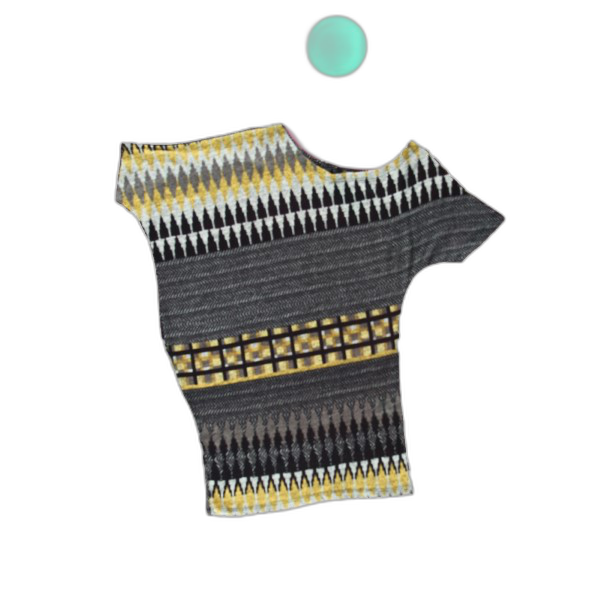
\includegraphics[width=.15\textwidth,height=50px]{./img/a}\hfill
		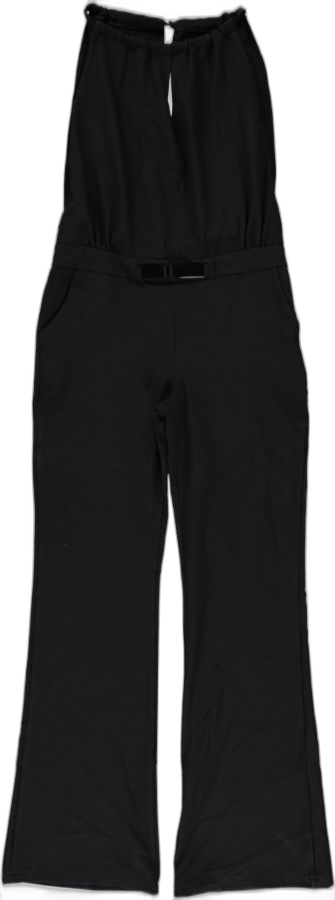
\includegraphics[width=.11\textwidth,height=70px]{./img/b}\hfill
		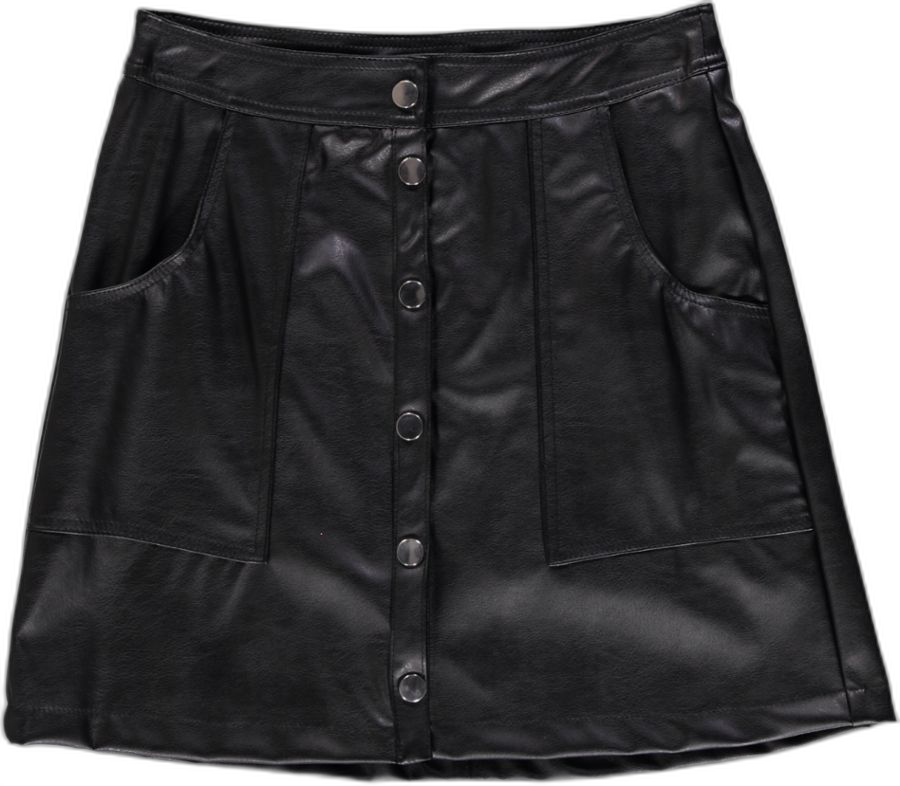
\includegraphics[width=.15\textwidth,height=50px]{./img/c}\hfill
		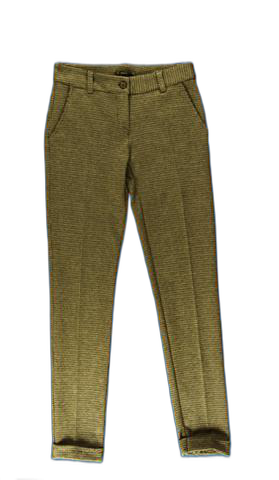
\includegraphics[width=.11\textwidth,height=70px]{./img/d}\hfill
		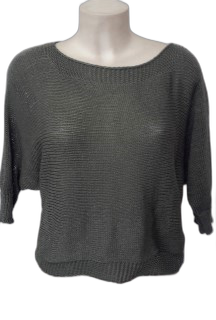
\includegraphics[width=.13\textwidth,height=70px]{./img/e}\hfill
		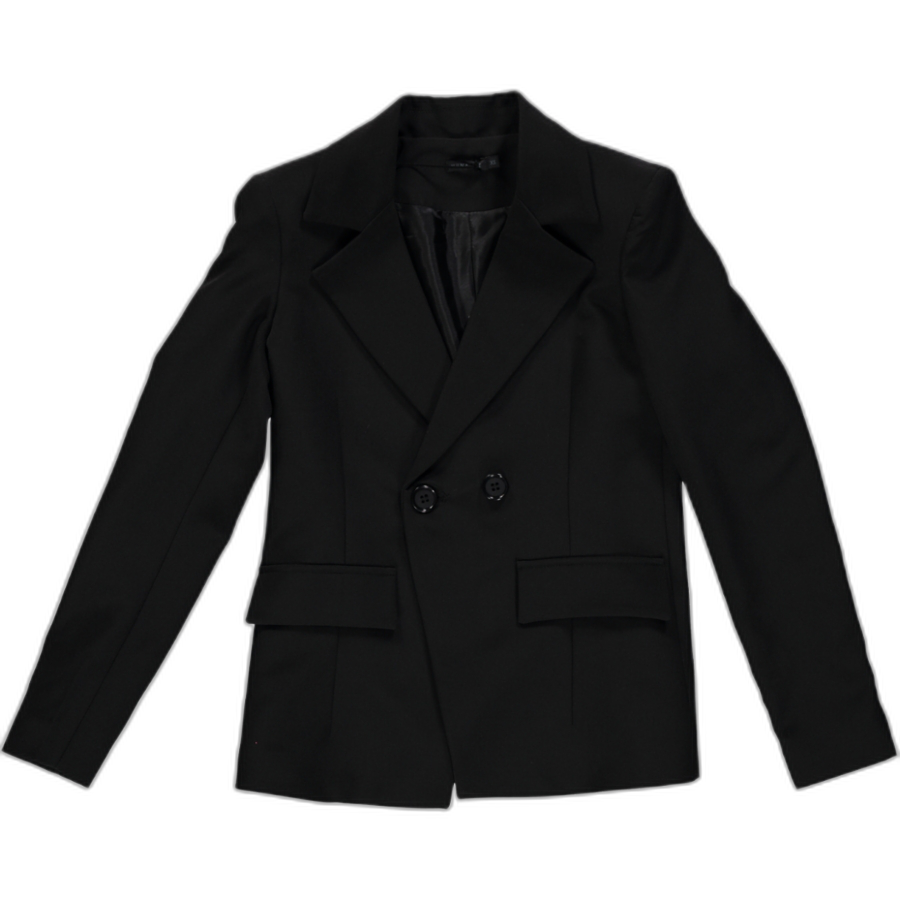
\includegraphics[width=.15\textwidth,height=70px]{./img/f}
	\end{figure*}

	Un elemento importante da considerare è il fatto che le immagini non hanno, originariamente, uguale dimensione. Per renderle processabili si è quindi scelto di caricarle sotto forma di immagini in scala di grigi di dimensione $256\times256$. \\
	Non avendo a disposizione delle labels precise su cui fare affidamento, si è deciso di analizzare il dataset per intero e valutare i risultati da un punto di vista qualitativo estraendo, per ogni cluster trovato, un immagine-media e valutandone la "mappabilità" in una categoria di indumenti generale nota. L'approccio utilizzato ha comportato l'ignorare eventuali outlier e incongruenze tra le immagini (es. presenza di manichino, orientamento differente...) considerando, qunidi, l'intero blocco di immagini come una black-box con cui lavorare e dalla quale estrarre informazione utile. \\
	A questo proposito sono state implementate varie tecniche di Feature-Extraction e Clustering che verranno discusse di seguito: l'idea è stata quella di avere più combinazioni per il processing dei dati al fine di analizzare il dataset secondo work-flow differenti per poter confrontarne i risultati finali e scegliere il più soddisfacente.
	
 

\chapter*{\huge Features Extraction}

	L'obbiettivo di questa fase è stato quello di estrarre dei vettori di features da ogni istanza dal dataset. L'idea di applicare un algoritmo di clustering direttamente alle immagini è infatti impraticabile considerando la dimensione eccessiva che avrebbero i vettori così ottenuti. Si è scelto di non adottare l'approccio banale di ridurre ancor più la dimensione delle immagini (fino a renderle trattabili) poiché i vettori risultanti sarebbero stati sicuramente poco interessanti e si sarebbe persa probabilmente molta informazione. In definitiva si è scelto di sfruttare, per l'estrazione delle features, le tecniche della PCA e delle Bag Of Words. 

\section*{PCA: Eigenfaces}

	Eseguire la PCA (Principal Component Analysis) su un dataset di immagini è di per se un task assai oneroso. La versione standard di questa tecnica, infatti, suppone che i dati seguano una distribuzione Gaussiana e prevede il calcolo della relativa matrice di covarianza $\Sigma = E[(x-\mu)(x-\mu)^{T}]$ con $x$ vettore istanza e $\mu$ vettore media entrambi di dimensione, nel nostro caso, $256\times256 \equiv 65536\times1$. Ne risulta una matrice di covarianza di dimensioni $65536\times65536$: troppo grande per essere gestita. Inoltre, l'operazione principale su cui si basa PCA, è il calcolo degli autovalori e autovettori della matrice, calcolo che risulta assai dispendioso date le sue dimensioni. 
	
	Trovare autovalori e autovettori è, di fatto, fondamentale poiché sappiamo dalla teoria che, prendendo i $k$ autovettori con autovalore più grande, si genera uno spazio delle features a ridotta dimensionalità nel quale proiettare le immagini del dataset in modo da ottenere vettori più piccoli. Il vantaggio di scegliere gli autovettori con autovalore più grande è legato al loro significato geometrico rispetto a $\Sigma$. Essi ne indicano infatti le direzioni di massima dispersione; ossia gli assi rispetto ai quali i punti del dataset che hanno generato la matrice di covarianza sono più sparsi (variano maggiormente). Pertanto, proiettando i dati originali sugli assi di questo spazio si otterrà una rappresentazione massimamente sparsa (wrt $k$) dei dati stessi e che quindi trattiene, quanto più possibile, l'informazione circa la distinguibilità dei punti. 
	
	Questo punto d'arrivo è fortunatamente raggiungibile anche per dataset di immagini sfruttando la variante della PCA detta Eigenfaces. Questa ci obbliga però ad accontentarci di un limite massimo imposto alla dimensionalità dello spazio ridotto il quale non potrà avere dimensione maggiore del numero di immagini del dataset.
	Questa tecnica consiste infatti nel "bai-passare" il calcolo della matrice $\Sigma$ calcolandone un'altra $\Gamma$ corrispondente alla matrice di covarianza del dataset avente cardinalità pari al numero delle feature ($65536$) ma con vettori di feature di lunghezza pari al numero di istanze nel dataset originale ($8890$). Questo dataset si ottiene semplicemente ragruppando le immagini (in formato vettoriale) in una matrice $D_{8890\times65536}$ e facendone la trasposta $D^{T} = A$. Ogni riga della matrice risultate sarà un elemento del nuovo dataset del quale dobbiamo calcolare la matrice di covarianza $\Gamma$. Da questa si potranno estrarre degli autovettori $\tilde{e}$ con determinate interessanti proprietà espresse di seguito:
	\begin{itemize}
		\item per ogni autovettore $\tilde{e}$ di $\Gamma$ esiste un autovettore $e$ di $\Sigma$ con ugual autovalore; 
		\item è possibile ricavare da $\tilde{e}$ il corrispondente autovettore in $\Sigma$ applicando: $e = A\tilde{e}$ (si suppone che in $A$ sia già stata sottratta la media);
		\item gli autovalori relativi ad autovettori di $\Sigma$ {\bf non} mappabili in un autovettore di $\Gamma$ avranno autovalore minore o uguale al più piccolo autovalore tra quelli di $\Gamma$.
	\end{itemize}
	Grazie a queste proprietà è stato possibile ricavare facilmente i primi $8890$ autovettori di $\Sigma$ sfruttando una ben più piccola matrice $\Gamma_{8890\times8890}$. Di questi sono stati selezionati i primi 32 al fine di generare il sottospazio nel quale proiettare il dataset. La scelta del valore 32 è legata al fatto che si è voluto mantenere un certo livello di comparabilità tra le performance di questa tecnica e quella trattata nel paragrafo seguente. L'algoritmo usato per implementare Bag of Words si è rivelato, infatti, particolarmente pesante al punto che non è stato possibile generare vettori di features di lunghezza maggiore a $32$. 
	
	Una proprietà interessante degli autovettori $e$ così ottenuti è il fatto che possono essere visualizzati, a loro volta, come immagini. Da queste è possibile intuire qualitativamente quali sono i dettagli ad alto livello che i relativi autovettori (assi del nuovo spazio a dimensione ridotta) vanno ad individuare. Di seguito si propongono i primi 5 autovettori estratti dall'algoritmo. \\
	\begin{figure*}[ht!]
		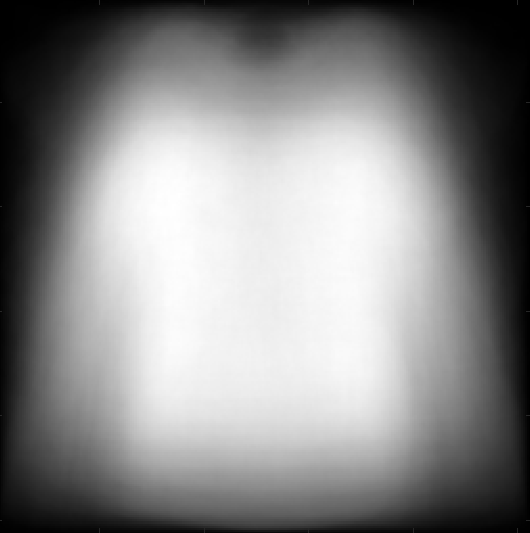
\includegraphics[width=.195\textwidth,height=80px]{./img/pca1}\hfill
		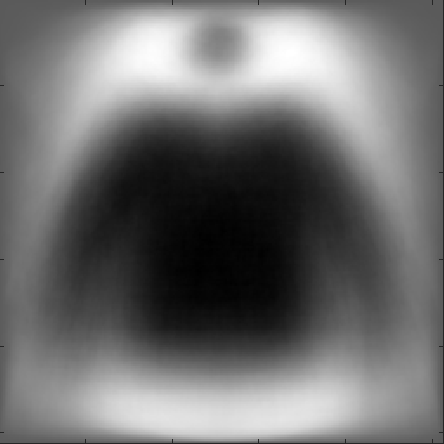
\includegraphics[width=.195\textwidth,height=80px]{./img/pca2}\hfill
		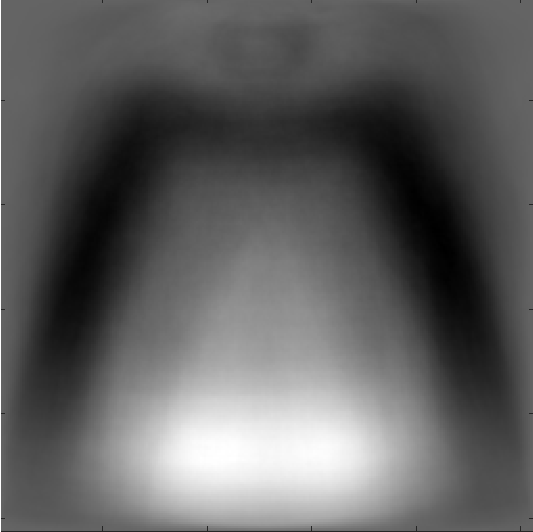
\includegraphics[width=.195\textwidth,height=80px]{./img/pca3}\hfill
		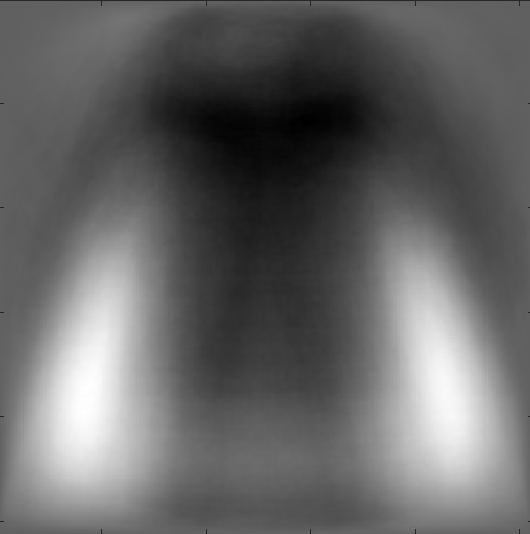
\includegraphics[width=.195\textwidth,height=80px]{./img/pca4}\hfill
		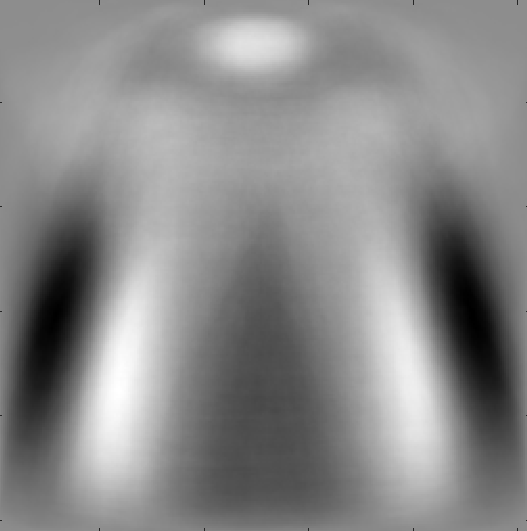
\includegraphics[width=.195\textwidth,height=80px]{./img/pca5}
	\end{figure*} 
	\\
	Da questi si possono già contraddistinguere alcuni elementi interessanti come la maschera di una maglia, di un pantalone, delle maniche lunghe e quella che potrebbe essere, in figura centrale, la maschera di una gonna. 
 
	Usando l'autovalore come "indice di informazione trattenuta" è possibile tracciare una curva che indichi la percentuale di sparsità che si è mantenuta applicando PCA e prendendo i primi $32$ autovettori per generare il sottospazio a più bassa dimensionalità. Questa percentuale, calcolata tramite la somma cumulativa normalizzata degli autovalori relativi ai primi $8890$ autovettori, non si basa, però, sul totale reale degli autovettori della matrice $\Sigma$. Tuttavia, all'atto pratico, il contributo dato a questa somma cumulativa dagli autovalori con indice $i$ (grande) è sempre più ininfluente man mano che $i$ cresce (l'indice in questione è quello relativo alla lista ordinata in senso decrescente degli autovalori stessi). Detto questo, possiamo dirci convinti del fatto che la percentuale stimata non sia troppo diversa da quella che si otterrebbe se si considerassero tutti gli autovalori. 
	Nel nostro caso, proiettando i vettori originali in uno spazio 32-D, abbiamo mantenuto, come mostra la seguente immagine, il $78\%$ circa dell'informazione.   
	\begin{figure*}[ht!]
	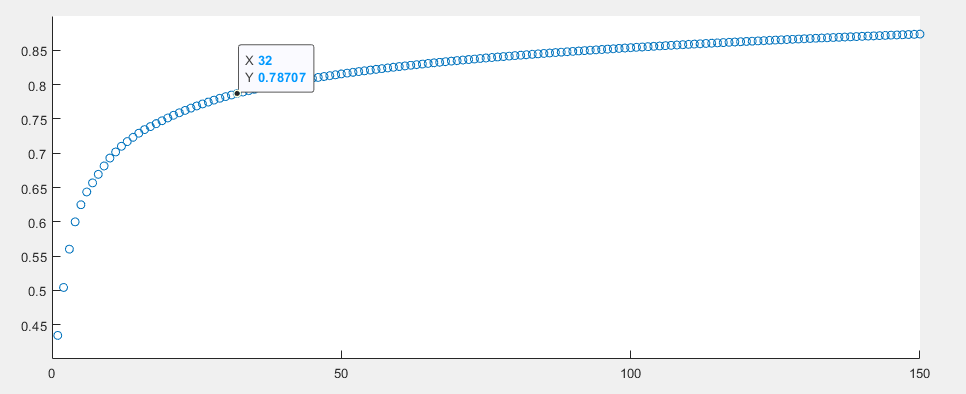
\includegraphics[width=\textwidth,height=200px]{./img/cum}
	\end{figure*}
	

\section*{Bag Of Words}	    

	La tecnica delle Bag of Words consiste nell'estrarre le features dalle immagini sfruttando un dizionario di "parole". La cardinalità di questo dizionario determina la lunghezza del vettore di features che contraddistinguerà ogni immagine. Quest'ultimo viene costruito computando, data una figura, il relativo istogramma delle parole ottenuto contando quanti descrittori dell'immagine sono mappabili in ciascuna word. Va definito ora cosa sono i descrittori e cosa si intende per mappabilità di questi rispetto alle parole.
	
	I primi non sono alto che vettori di valori specifici per il tipo di istanze che si sta trattando. Possono essere ottenuti tramite vari metodi e possono avere determinate proprietà come, per esempio, l'invarianza rispetto a particolari trasformazioni. Nel nostro caso sono stati utilizzati i descrittori più semplici ottenuti applicando la tecnica Regular Grid. In questo caso i vettori sono patch $32\times32$ estratti dall'immagine secondo una griglia che la divide in sezioni di tale dimensione. La seguente immagine mostra la griglia che individua e divide i vari patch all'interno dell'immagine: questa è solo d'esempio, i patch in questione non sono di dimensione $32\times32$ (ogni immagine del dataset è stata, infatti, tessellata in $64$ sezioni).
	\begin{figure*}[ht!]
		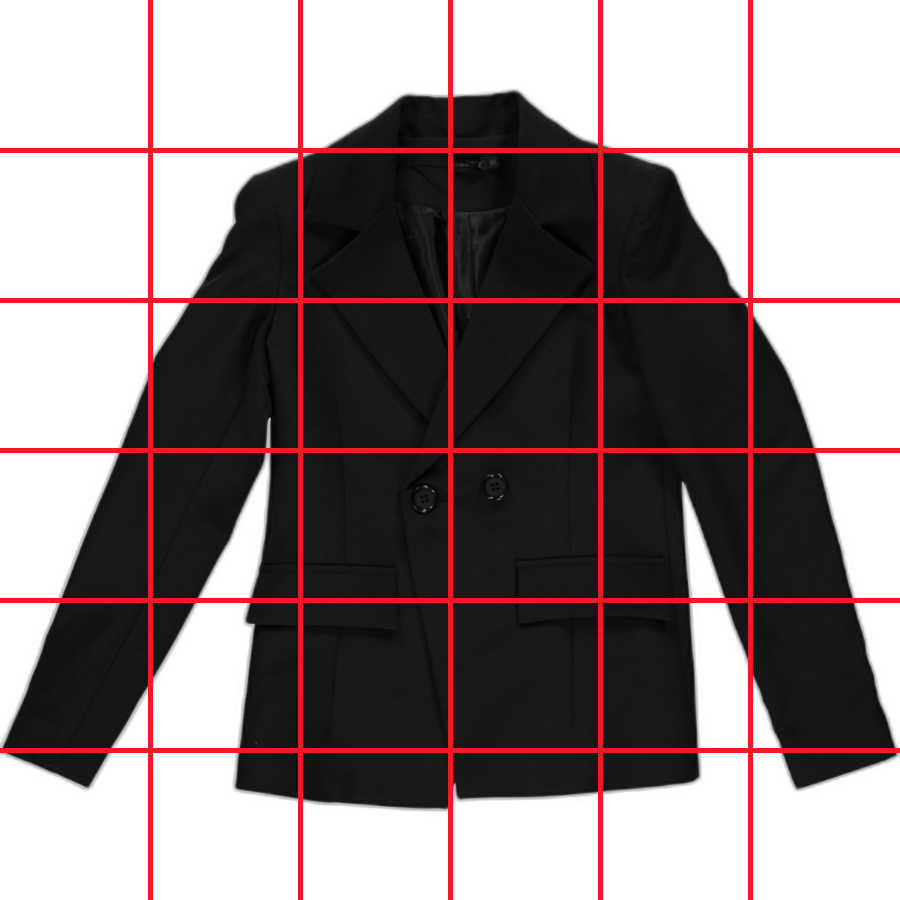
\includegraphics[width=120px,height=120px]{./img/patch}
		\centering
	\end{figure*}
	
	Per definire il concetto di mapping tra patch e parole occorre prima dettagliare la struttura del dizionario e come questo viene costruito. Per ottenere questo oggetto è necessaria una fase di Dictionary Learning in cui si generano le parole che ne costituiscono il contenuto. Esistono svariati modi per ottenere queste parole ma ,in generale, quello che si fa è prendere i descrittori ottenuti dall'intero dataset ed eseguire qualche tipo di calcolo al fine di ottenerne un numero fissato (generalmente inferiore) da utilizzare come set di parole. A seconda del contesto, questa operazione (come quella di mapping) può essere eseguita con metodi diversi. Nel nostro caso si è deciso di applicare l'algoritmo  {\bf{ \it K-Means}} con $K = 32$ per ottenere $32$ parole (e di riflesso istogrammi di features di lunghezza pari a $32$). Da notare che non c'è nessuna attinenza tra questo valore e la dimensione dei patch delle immagini: è stato scelto in entrambi i casi il valore 32 per ragioni legate alla complessità dell'algoritmo e alla grandezza del dataset. Infatti, con questi parametri, {\bf{ \it K-Means}} si ritrova a lavorare con $64\times8890$ istanze di lunghezza $32\times32 = 1024\times1$ da clusterizzare in $32$ medie. L'algoritmo impiega tanto più tempo a convergere quante più sono le medie da calcolare e quanto più piccole sono le dimensioni del patch: i valori stabiliti hanno fatto si che fosse possibile ottenere un numero di parole significativo in tempi ragionevoli (seppur molto lunghi: $\sim2$ ore). Alcuni esempi di parole estratte dall'algoritmo sono le seguenti:
	\begin{figure*}[ht!]
		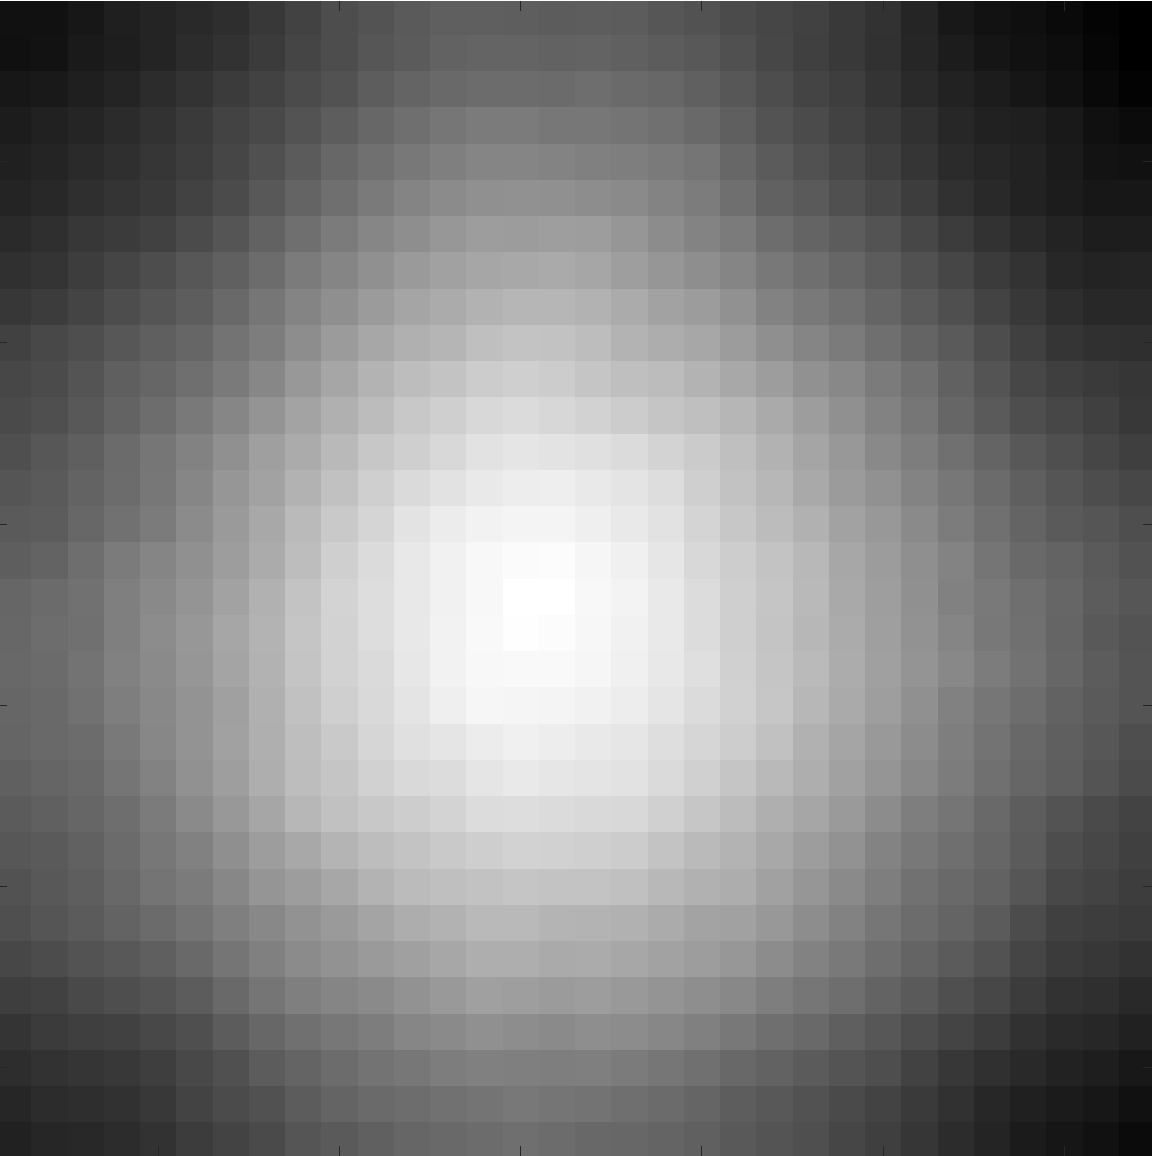
\includegraphics[width=.16\textwidth,height=70px]{./img/bow1s}\hfill
		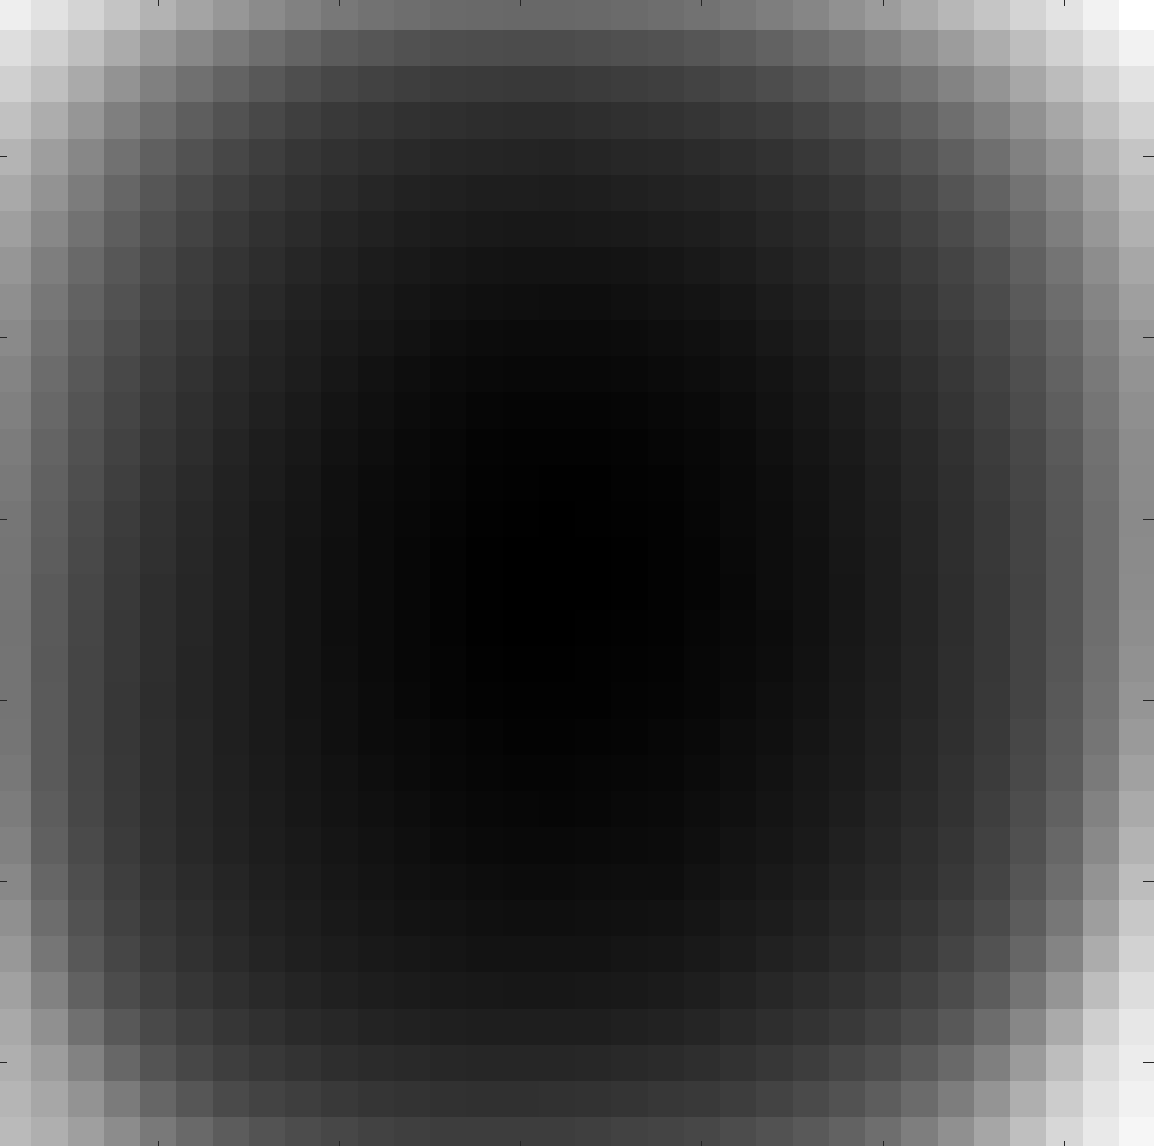
\includegraphics[width=.16\textwidth,height=70px]{./img/bow2s}\hfill
		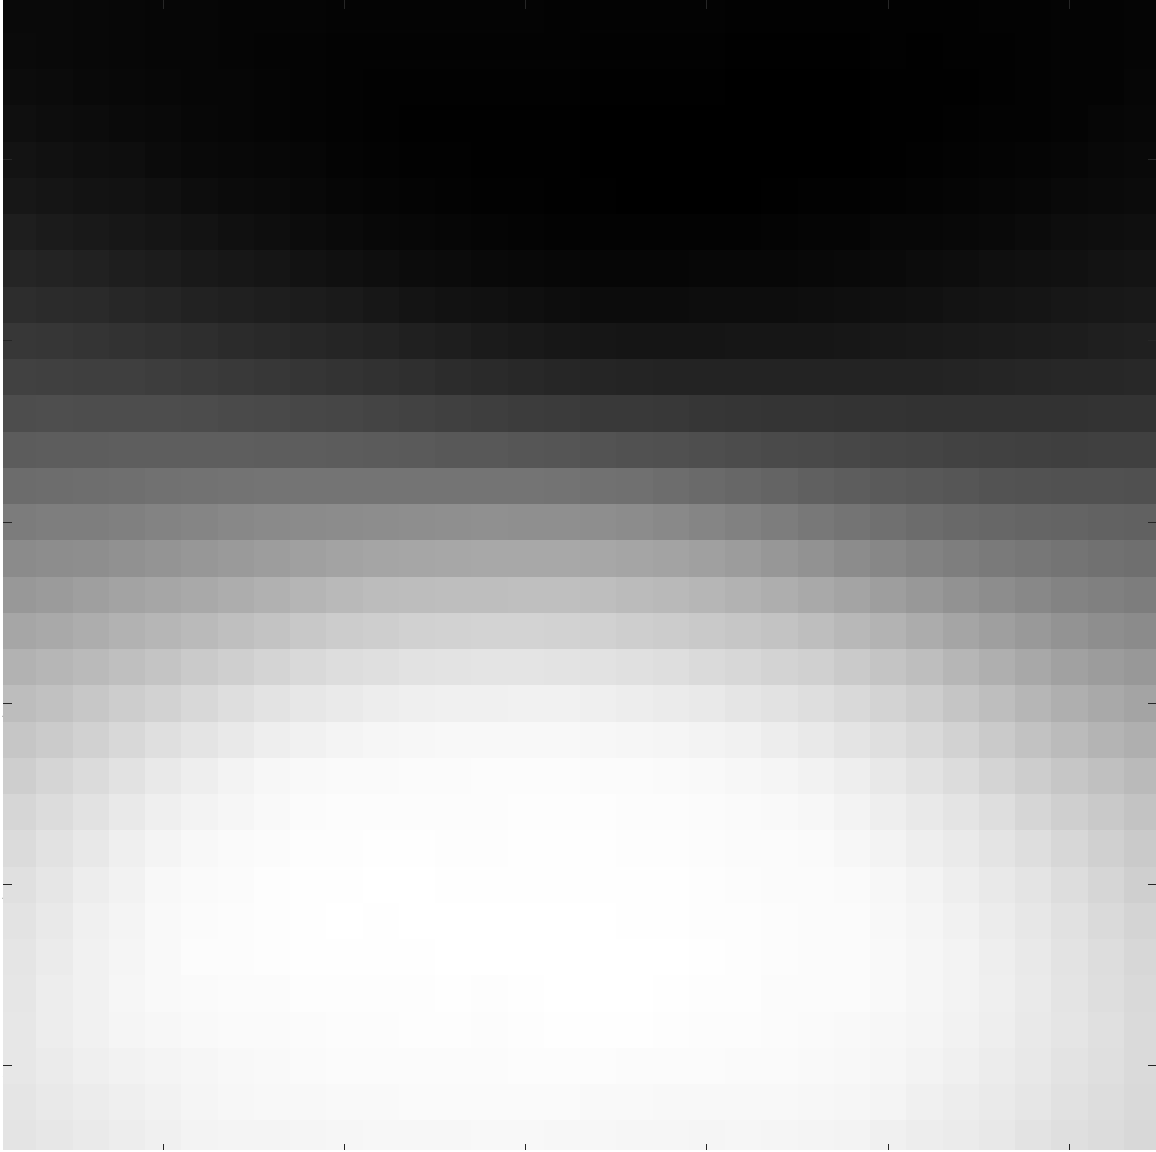
\includegraphics[width=.16\textwidth,height=70px]{./img/bow3s}\hfill
		
\includegraphics[width=.16\textwidth,height=70px]{./img/bow4s}\hfill
		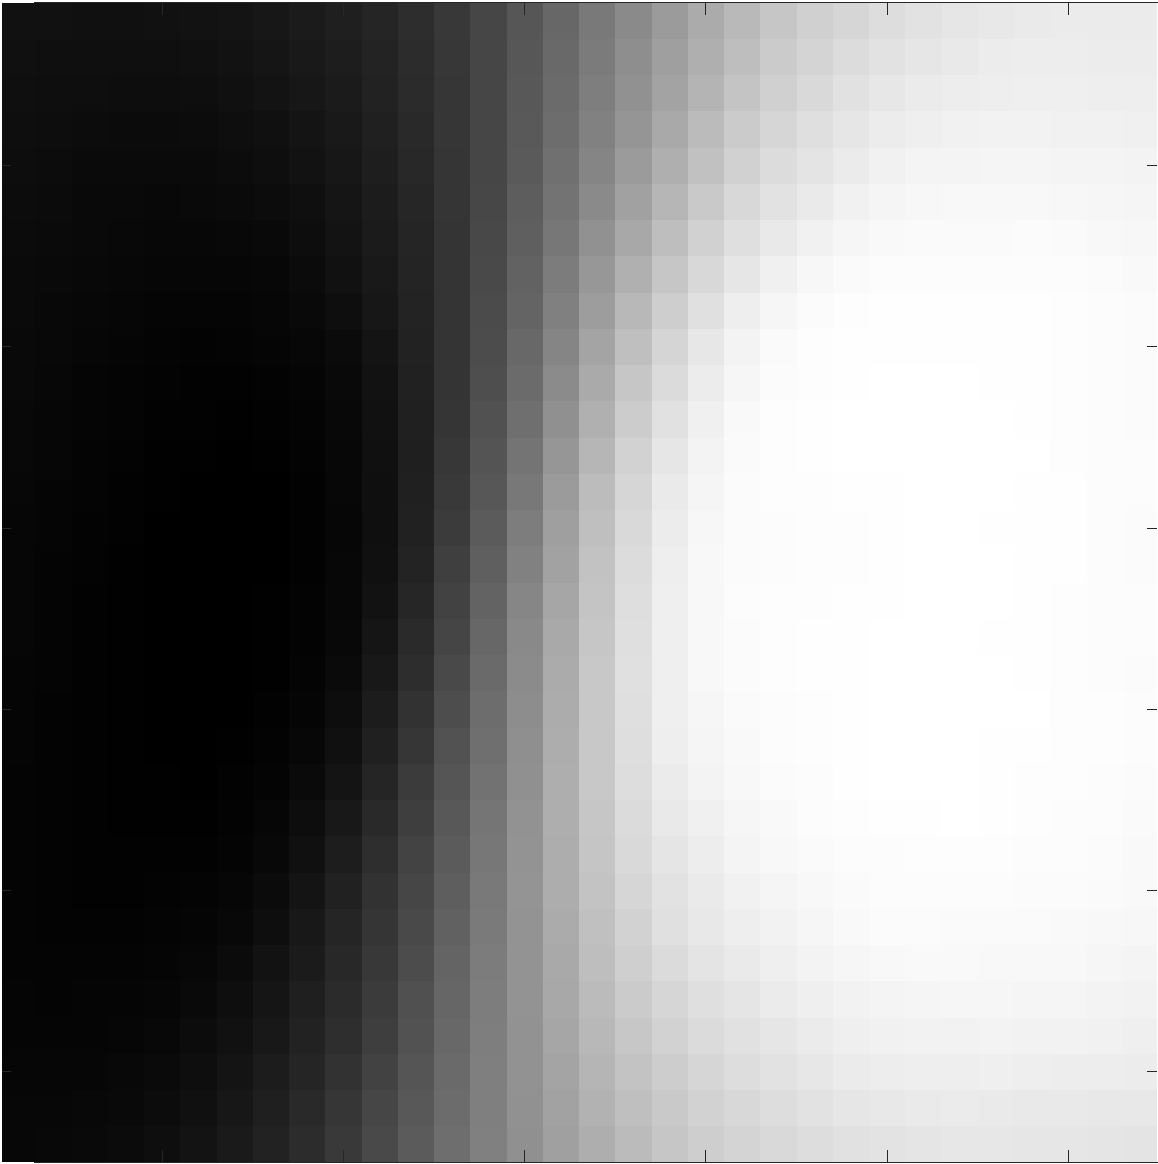
\includegraphics[width=.16\textwidth,height=70px]{./img/bow5s}\hfill
		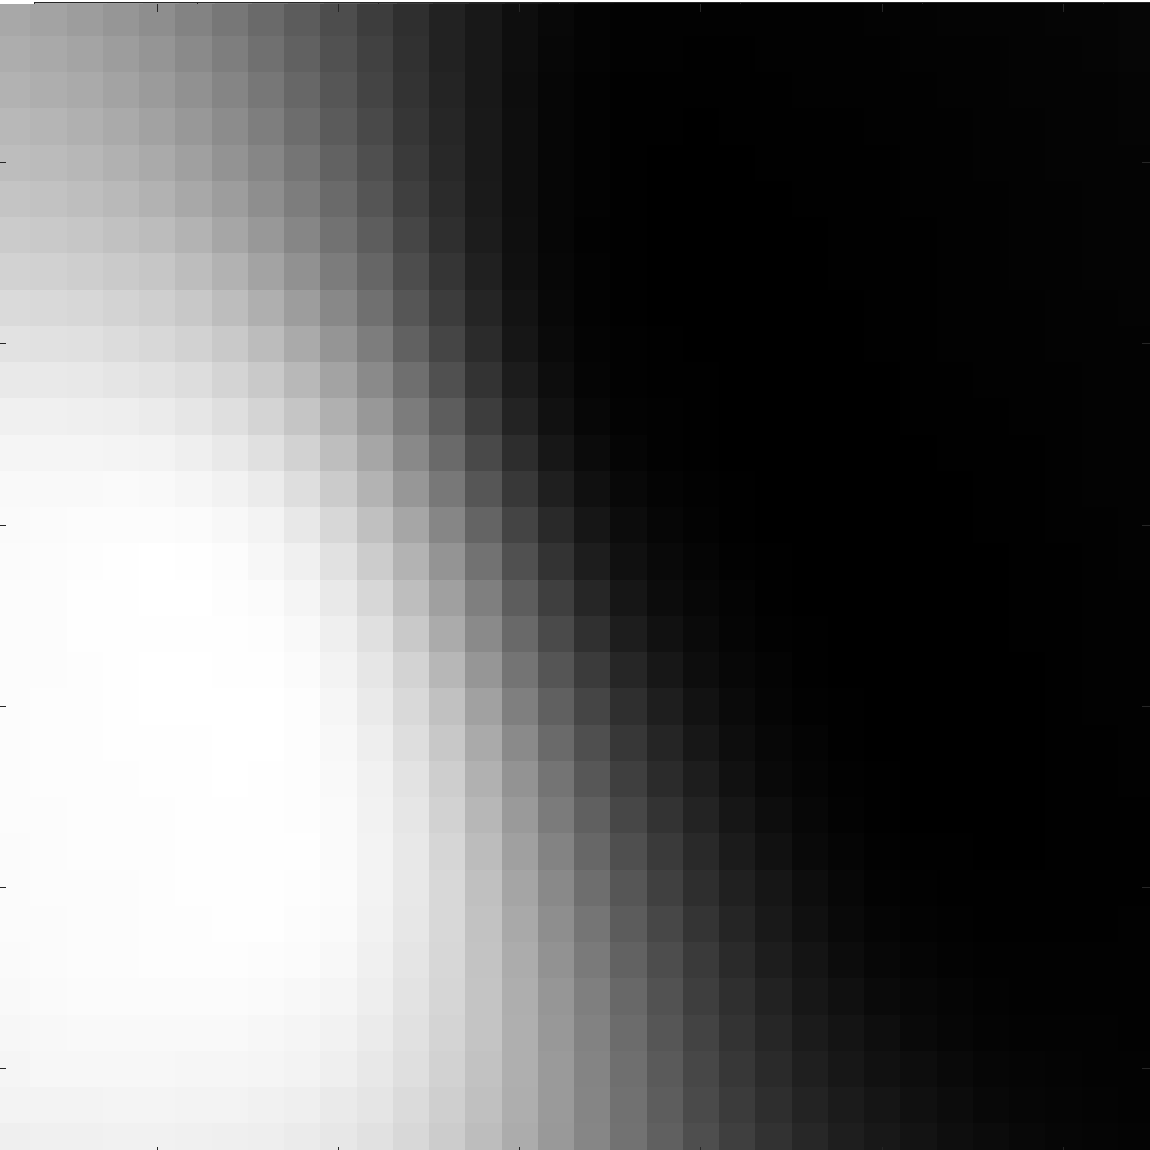
\includegraphics[width=.16\textwidth,height=70px]{./img/bow6s}
	\end{figure*} 
	
	Costruito il dizionario occorre, quindi, stabilire un metodo per associare ogni patch di una data immagine alla relativa parola. Si è quindi scelto di mappare ogni patch nella parola del dizionario avente distanza Euclidea inferiore. E' stato possibile applicare agevolmente questa misurazione dal momento che entrambi questi elementi, per costruzione, hanno la stessa misura. 
	
	Un altro elemento da sottolineare è il fatto che, nel codice, si è in realtà deciso di calcolare $31$ medie/parole invece che $32$. Questo perché tutti gli "almost-0-patch" sono stati esclusi dalla computazione ed associati, in fase di embedding (calcolo istogrammi), ad una 32-esima word aggiunta appositamente. Questi patch particolari sono stati identificati in fase di tessellatura delle immagini e corrispondono a vettori dove meno di $1/32$ dei valori non sono zeri. Questa scelta è stata fatta al fine di alleggerire il calcolo delle medie ed è supportata dal fatto che le immagini degli abiti sono in realtà delle maschere. Quando Matlab le carica, infatti, si può notare come, esternamente alla figura del vestito, vi siano solo valori nulli. La threshold $1/32$ (hardcoded e ad-hoc rispetto al task di riferimento) è stata scelta in modo da escludere dal calcolo solo i patch effettivamente poco interessanti ma mantenere quelli che conservavano (almeno) un certo quantitativo minimo di informazione. 

	Per concludere, va ricordato che, essendo l'output dell'algoritmo fortemente dipendente dai $K$ centri che si scelgono in fase di inizializzazione di {\bf{ \it K-Means}}, i risultati discussi in questo elaborato potrebbero non essere riprodotti fedelmente dalla ri-esecuzione del codice. A questo proposito, i dati restituiti da questo algoritmo ed utilizzati per gli step successivi, sono stati salvati così da poterli ricaricare se si volesse riprodurre fedelmente l'esecuzione del codice qui discussa. 
	

\chapter*{\huge Clustering}

	In questa fase della computazione l'obbiettivo è stato quello di ottenere dei cluster di immagini che fossero semanticamente simili. Di seguito verranno descritti, in particolare, gli algoritmi utilizzati; si rimanda al capitolo successivo la discussione dei risultati ottenuti. Per il clustering sono stati scelti l'algoritmo standard di Expectation-Maximization, BSAS e l'algoritmo di Mean Shift.  
	

\section*{Expectation Maximization}

	L'algoritmo di Expectation-Maximization è un algoritmo relativamente semplice che ci permette di ottenere buoni risultati nei problemi di clustering dove lo applichiamo. Questo algoritmo ha come obbiettivo quello di ottenere, in merito ad una distribuzione di punti espressi in forma vettoriale, un numero $K$ di blob gaussiani ciascuno descritto da una matrice di covarianza e una media (entrambe restituite dall'algoritmo). 
	Nell'applicare questa tecnica di clustering, infatti, si suppone che i dati siano distribuiti secondo una Gaussiana Multimodale: ciò che si vuole trovare è, in altri termini, una superficie di separazione che ci permetta di associare i punti alle rispettive mode. 
	Anche in questo caso le performance e i risultati sono fortemente influenzati dal parametro $K$ (numero mode) che si sceglie e dal come si inizializzano i parametri dei vari cluster nella fase di set-up preliminare. 
	
	L'algoritmo di clustering che sfrutta questo metodo è quindi un algoritmo di stima dei parametri e si può categorizzare come partizionale e model-based in quanto genera una singola divisione dei dati basata sui modelli (blob gaussiani) che astrae direttamente da questi. Tra le altre caratteristiche interessanti troviamo il fatto che è un algoritmo non incrementale e tipicamente hard (pattern/istanze assegnate ciascuna ad un solo cluster).   
	
	Questa tecnica prevede l'alternarsi di due fasi di calcolo: una di expectation, nella quale avviene la stima di una funzione di likelihood che definisce la probabilità di appartenenza di un dato punto ai vari cluster, e una di maximization in cui si aggiornano i parametri del modello in base alle probabilità calcolate nello step precedente.  
	Il codice che implementa questa tecnica fa uso del logaritmo di queste funzioni, poichè, all'atto pratico, si lavora spesso con probabilità anche molto piccole e, per non rischiare l'underflow, conviene adottare questo trick che semplifica i calcoli e non invalida l'algoritmo. 
	Matematicamente, quello che si vuole calcolare, è, omettendo i logaritmi, la classica formula di Bayes espressa come segue:
	$$ P(C_j|x_i) = \frac{ P(x_i|C_j)P(C_j)}{\sum_{j} P(x_i|C_j)P(C_j)} $$
	Data $D$ cardinalità del dataset e $N(\mu,\Sigma)$ distribuzione normale sulla media $\mu$ e matrice di covarianza $\Sigma$, è possibile definire i seguenti elementi: 
	$$ \begin{matrix}
		P(x_i|C_j) = N(x_i|\mu_j,\Sigma_j) & ~~~~~~~ & P(C_j) = \frac{\sum_{j} P(C_j|x_i)}{D}
	\end{matrix}$$ 
	Definiti questi strumenti si può ora comprendere cosa accade nella fase di expectation: partendo dal presupposto di avere a disposizione la stima dei parametri $\mu$ e $\Sigma$ per ogni cluster e aver già calcolato, in qualche modo, una stima di $P(C_j)$, è necessario calcolare ora $P(C_j|x_i)$ sfruttando, banalmente, le formule definite sopra.
	Nella fase di maximization si utilizzerà la funzione $P(C_j|x_i)$ appena stimata per ricalcolare i parametri stessi del problema. In particolare, per l'aggiornamento dei parametri $\mu$ e $\Sigma$ (per $P(C_j)$ si usa la formula definita prima), si potranno utilizzare le seguenti:
	$$ \begin{matrix}
		\mu_j = \frac{\sum_{i} P(C_j|x_i)x_i}{\sum_{i} P(C_j|x_i)} & ~~~~~~~ & \Sigma_j = \frac{\sum_{i} P(C_j|x_i)(x_i-\mu_j)(x_i-\mu_j)^{T}}{\sum_{i} P(C_j|x_i)}
	\end{matrix}$$ 

	Punto focale dell'algoritmo è l'utilizzo della stessa likelihood come funzione di pesi attribuiti ad ogni istanza del dataset nel calcolo dei parametri relativi ai vari blob gaussiani. Questo fatto ci permette di ripetere ciclicamente i passi di expectation e maximization fino ad arrivare a convergenza. Questa, nel nostro caso, è determinata dal valore ottenuto sottraendo il valore di $llh(i)$ a $llh(i-1)$. Se questa differenza restituisce un risultato inferiore ad un certo valore di soglia l'algoritmo termina. La variabile $llh$ conserva, ad ogni iterazione $i$ del main loop dell'algoritmo, il valore medio calcolato sul vettore $T$ contenente i valori del logaritmo della seguente funzione $\sum_{j} P(x_i|C_j)P(C_j)$ (denominatore di $P(C_j|x_i)$). Questa media attesta la "bontà" dei parametri sin ora stimati e tende ad assestarsi ad un massimo (locale) il quale, se raggiunto, comporta la terminazione dell'algoritmo.
	   
	  	
\section*{Mean Shift}

	Mean Shift è un altro interessante algoritmo di clustering utilizzato nel contesto del {\it Non Parametric Density Learnign}. Mean Shift esegue un clustering di tipo partizionale, hard e non incrementale. Il codice utilizzato per implementare questa tecnica semplifica molto l'intero calcolo previsto dall'algoritmo e, talvolta, esegue merge di cluster esistenti con quelli appena trovati: considerando questo aspetto, si può dire che la funzione utilizzata nel progetto segue anche un approccio agglomerativo (non è possibile, però, generalizzare in quanto Mean Shift non è, di base, agglomerativo). 
	
	Questa tecnica prende spunto dall'algoritmo di Parzen Windows che mira a descrivere la distribuzione dei punti che si sta analizzando andando a guardare l'intorno degli stessi. Parzen Windows raggiunge questo obbiettivo partendo dal presupposto che tutti i punti appartengano alla stessa classe e che la probabilità di trovare un elemento in un determinato punto dello spazio sia tanto più grande quanti più punti si trovano nel suo intorno. Definito quindi un raggio $h$ che sancisce il limite dell'intorno e un valore $N$ corrispondente alla cardinalità del dataset, sarà sufficiente calcolare la seguente formula per ottenere la probabilità desiderata: $ P(x) = \frac{1}{N}\sum_{i=1}^{N}K((x-x_i)/h)$.  La variabile $h$, che non appare direttamente nella formula, agisce quindi solo sull'input della funzione kernel $K$. Quest'ultima restituisce un peso a seconda del vettore $d$ che riceve in input il quale rappresenta, a sua volta, il vettore di collegamento tra il punto $x$ e $x_i$ diviso per $h$. Le funzioni kernel sono sì arbitrarie, ma devono rispettare alcune proprietà tra cui: restituire valori reali e $\geq 0$, integrare ad $1$, essere simmetriche e avere massimo in $0$. Tra le funzioni kernel più utilizzate abbiamo quella di Epanechnikov, quella Normale e quella Uniforme. Nonostante quanto appena detto si riferisca specificatamente all'algoritmo Parzen Windows, questo stesso concetto di kernel viene ripreso anche da Mean Shift: nel nostro caso si utilizza un kernel uniforme il quale opera secondo la seguente:
	
	$$ K(d) = \bigg\lbrace \begin{matrix}
		1 & if~||d||\leq1 \\
		0 & otherwise
	\end{matrix}$$        
	
	Mean Shift, nello specifico, non ha come obbiettivo quello di individuare una distribuzione di probabilità bensì quello di definire superfici di divisione nello spazio dei punti. Per farlo cerca di associare massimi locali di $P(x)$ ai punti del dataset computando, a partire da ciascun punto, un path che li colleghi al corrispettivo massimo. Questo path viene calcolato seguendo il gradiente di $P(x)$ ottenuto tramite la seguente formula:
	$$ \nabla P(x) = \frac{1}{N}\sum_{i=1}^{N}\nabla K((x-x_i)/h) = \frac{1}{N} \left[ \sum_{i=1}^{N} g(d_i) \right] \left[\frac{\sum_{i=1}^{N} x_i g(d_i)}{\sum_{i=1}^{N} g(d_i)} - x \right]$$
	con $g(d_i)$ corrispondente alla derivata prima di $-k(||d_i||^2)$ ossia alla versione 1-D di $K$. 
	All'atto pratico ci si concentra sul secondo membro di questa formula il quale si può vedere geometricamente come il vettore che collega il punto analizzato al centro di massa della window attuale il quale si ottiene dalla media pesata $m= (\sum_{i=1}^{N} x_i g(d_i))/(\sum_{i=1}^{N} g(d_i))$ . La window si può definire come sezione di spazio entro la quale i punti vengono considerati dal kernel (legata ad $h$).  
	Muovendoci lungo questo vettore verso il centro di massa e ricalcolando, ad ogni spostamento, la formula, si otterrà un path che ci farà avvicinare sempre più al massimo locale di $P(x)$ al quale associare $x$. Questo path garantisce, ammettendo passi infinitesimali, la convergenza al massimo locale. Nella pratica, per stabilire la convergenza, si impone una threshold al modulo del vettore-spostamento al di sotto della quale l'algoritmo termina. Si dimostra infatti che la grandezza del modulo tende a $0$ man mano che ci si avvicina al massimo.
	
	Facendo partire l'algoritmo da ogni punto del dataset si otterrà, quindi, una serie di massimi locali che identificano i cluster di interesse. Per dataset grandi può risultare troppo oneroso eseguire la computazione per ogni punto. Nel codice utilizzato si è deciso di utilizzare il sistema "a voti" descritto in seguito per velocizzare i calcoli.
	   
	Essendo questo l'unico algoritmo non scritto da zero (o adattato da quelli visti a lezione) è doveroso proporne un'analisi più dettagliata.
	 
	Lo script parte inizializzando la variabile $bandSq$ al quadrato del valore $bandWidth$ (ricevuto come parametro) e salvando la lista di indici delle istanze ricevute in input. A questo punto ricava i valori massimi e minimi contenuti nel dataset rispetto ad ogni feature. Questi valori vengono utilizzati per stimare la grandezza dello spazio sul quale si sta operando calcolando la norma del vettore contenente la lunghezza dei lati della bounding box che definisce lo spazio di interesse. Sempre in questa fase viene inizializzata la threshold di convergenza a $1^{-5}$ volte il parametro di $bandWidth$.
	
	Ha inizio, poi, il loop principale che viene eseguito fino a quando tutti i punti non sono stati analizzati. A tenere traccia di questa analisi vi è un vettore apposito, lungo quanto l'intero dataset, i cui valori vengono utilizzati come flag ($1=analized$, $0=pending$). All'interno del loop viene scelto randomicamente un punto tra quelli interni al dataset (non ancora analizzato) e con esso si inizializza la media corrente. Si inizializza quindi un altro vettore $thsiClusterVotes$ rappresentante quante volte un dato punto del dataset è stato trovato in una delle windows (computate nel ciclo interno) nell'iterazione corrente.
	
	Successivamente si entra, quindi, nell'appena citato loop interno che termina solo a convergenza. Al suo interno, come primo step, viene calcolata la distanza di tutti i punti wrt la media corrente. Vengono quindi selezionati tutti i sample la cui distanza è minore di $bandSq$  e viene incrementato il relativo valore in $thisClusterVotes$. Viene quindi aggiornata la media interna alla window in analisi e vengono considerati come appartenenti al cluster corrente {\bf tutti} i punti interni ad essa. Questa è una semplificazione atta a velocizzare la computazione altrimenti troppo onerosa per dataset grandi. A questo punto, se la distanza tra vecchia e nuova media è minore della threshold (impostata in fase di inizializzazione) si esce dal ciclo interno. Prima di uscire dal loop si esegue un filtraggio dei risultati ottenuti. In particolare si cerca un merge del cluster attuale con quelli calcolati in precedenza usando come metro di misura la distanza tra le rispettive medie comparata ad una threshold corrispondente ad una frazione della $bandWidth$. 
	
	Una volta analizzati tutti i punti si esce dal ciclo e si salvano i risultati ottenuti dal clustering attribuendo ad ogni istanza del dataset la corrispettiva label. Questa viene scelta prendendo l'indice del cluster che ha ricevuto più voti (si controlla il vettore $clusterVotes$ incrementato di iterazione in iterazione da $thisClusterVotes$). 
	
	In conclusione va tenuto presente che, con questa tecnica, il numero di cluster ottenuto varia a seconda del parametro $h$ ($bandWith$) e non è possibile sceglierlo a priori. Un'aspetto interessante è anche il fatto che non si fa nessuna assunzione sulla distribuzione dei punti lasciando quindi più "libertà" all'algoritmo nella definizione dei cluster.	
	
	
\section*{BSAS}

	Questo algoritmo di clustering è probabilmente il più semplice tra quelli utilizzati per questo progetto: l'idea alla sua base consiste nel generare cluster analizzando ogni istanza del dataset una sola volta. Per farlo BSAS analizza il primo elemento e genera un cluster ad esso correlato. Questo cluster (come i seguenti) sarà descritto da una media e da una conta dei punti in esso inclusi. L'analisi dei successivi elementi risulta più complessa. Considerando il secondo elemento, bisognerà calcolarne la distanza con la media del primo cluster (euclidea nel nostro caso). Se questa non supera una certa soglia prefissata, si aggiunge il punto al cluster e si aggiornano i parametri (media e conta). Nel caso in cui la distanza superi la soglia si genererà un secondo cluster con media iniziale corrispondente al secondo elemento e con conta ad 1. Questo procedimento viene ripetuto per tutti gli elementi del dataset e restituirà un numero di cluster che, di base, non è decidibile a priori. BSAS è un algoritmo di clustering partizionale, hard e, avendo usato la media dei punti per identificare ogni cluster, incrementale.   
	
	Il codice di BSAS utilizzato nel progetto devia leggermente da quella che è la descrizione teorica appena data. Si è deciso infatti di modificare l'algoritmo in modo da limitare il numero di cluster che esso genera tramite un parametro di controllo ricevuto in input dalla relativa funzione. Dato un numero $k$ rappresentante il numero massimo di cluster, la funzione farà sì che, nel caso in cui l'algoritmo tenti di creare il $(k+1)$-esimo cluster, il processo di generazione dello stesso si interrompa e si opti, invece, per l'aggiornamento del cluster con distanza inferiore rispetto al punto analizzato.
	
	Questa modifica di BSAS, pur cambiando drasticamente il comportamento dell'algoritmo per $k$ piccoli, non ne degrada eccessivamente le performance e rispetta il principio cardine della tecnica (analisi di ogni pattern una sola volta). Inoltre si può ignorare il fatto che questo accorgimento vada a "premiare" gli elementi che vengono analizzati prima nella computazione poiché, per come è costruito, BSAS ha da sè un bias verso le prime istanze che elabora. Da questa osservazione si può notare un altra caratteristica di questa tecnica ossia il fatto che i risultati dipendono fortemente dall'ordine con cui si analizzano i vari sample: ordini diversi potrebbero generare prima cluster con medie anch'esse diverse e includere, quindi, elementi distinti. A questo proposito, per non complicare il codice, si è scelto di utilizzare come unico ordine di analisi quello utilizzato dal dataset.
	
	Quanto detto finora ha posto in secondo piano una questione che è in realtà cruciale per l'algoritmo: l'inizializzazione del parametro di soglia per la distanza punto-cluster. Si è scelto di inizializzare questo parametro alla metà della distanza dei punti del dataset massimamente lontani. Inoltre, facilitati dalla bassa complessità di BSAS, si è deciso di ripetere in un loop l'algoritmo diminuendo la soglia di $1/20$ (hardcoded) ad ogni iterazione fino ad arrivare a 0.
	
	 A fine funzione viene comunque restituito un solo risultato che viene scelto secondo un'euristica. Generalmente, quello che si tende a fare, è analizzare la funzione che tiene traccia del numero di cluster restituiti da BSAS (in funzione del parametro di soglia) alla ricerca di un plateau. Questo determinerà un intervallo di valori di soglia per i quali l'algoritmo restituisce un output simile e quindi (sperabilmente) più significativo in termini di custering. Il codice implementato fa uso invece di un altra euristica per decidere il risultato migliore poiché quella appena proposta non si adatta bene al contesto descritto (20 iterazioni sono poche per trovare un plateau). Quello che si è deciso di fare è valutare ogni risultato secondo la cardinalità dei cluster ottenuti. Per ogni applicazione di BSAS si computa infatti la cardinalità media che viene sottratta poi alla cardinalità di ogni cluster. Si fa quindi una media dei risultati (presi in modulo) al fine di ottenere un coefficiente di variazione. A questo punto si sceglierà il risultato che ha un coefficiente più basso ad indicare il fatto che i cluster ad esso relativi avranno cardinalità più simile. Questa euristica è stata utilizzata basandosi sul presupposto che ogni cluster dovesse contenere un numero all'incirca simile di elementi. Rispettando l'approccio "black-box" si è deciso di guardare le immagini del dataset solo dopo la progettazione dell'algoritmo. Alla luce dei dati da analizzare si è comunque ritenuta verosimile l'ipotesi circa la "cardinalità attesa dei cluster" fatta in fase di progettazione.   


\chapter*{\huge Risultati}

	Di seguito verranno esposti i risultati ottenuti dall'esecuzione di ogni algoritmo di clustering. Per ciascuno, verranno messi a confronto gli output calcolati rispetto alle due diverse tecniche di estrazione delle feature trattate in precedenza. 
	
	Per ciascun risultato verranno specificati i parametri dell'algoritmo utilizzati per ricavarlo. Ovviamente verranno mostrati solo i risultati ottenuti con i parametri migliori.  
	
	Per ogni computazione il numero di cluster prodotti è stato limitato ad un massimo di 25 per non eccedere nella generazione di raggruppamenti troppo specifici.
	
	\section*{Expectation Maximization}
	
	L'algoritmo di Expectation Maximization necessita, come detto in precedenza, di un valore $k$ corrispondente al numero di blob gaussiani da modellare. I risultati mostrati nelle figure sottostanti si riferiscono entrambi ad esecuzioni dell'algoritmo aventi $k = 25$.
	Già dall'output di questo algoritmo ci si accorge dell'enorme differenza in termini di performance presente tra i vettori di feature ottenuti tramite PCA da quelli ottenuti tramite la funzione Regular-Grid (Bag of Words).
	
	\begin{figure*}[ht!]
		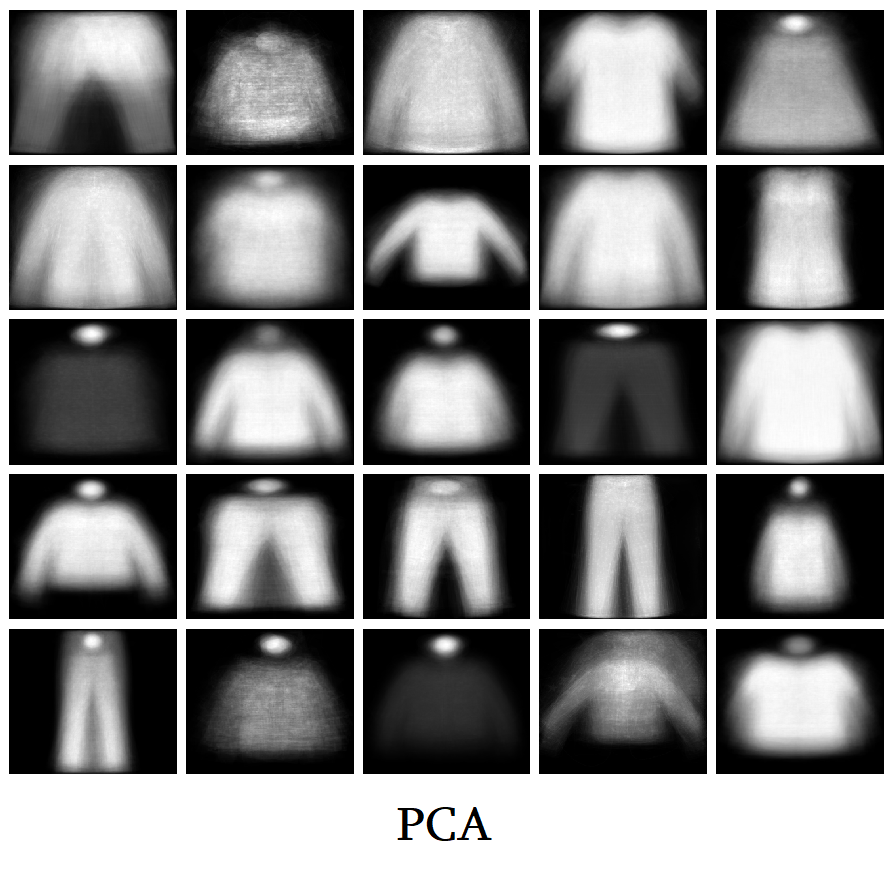
\includegraphics[width=.49\textwidth,height=250px]{./img/EM_PCA}\hfill
		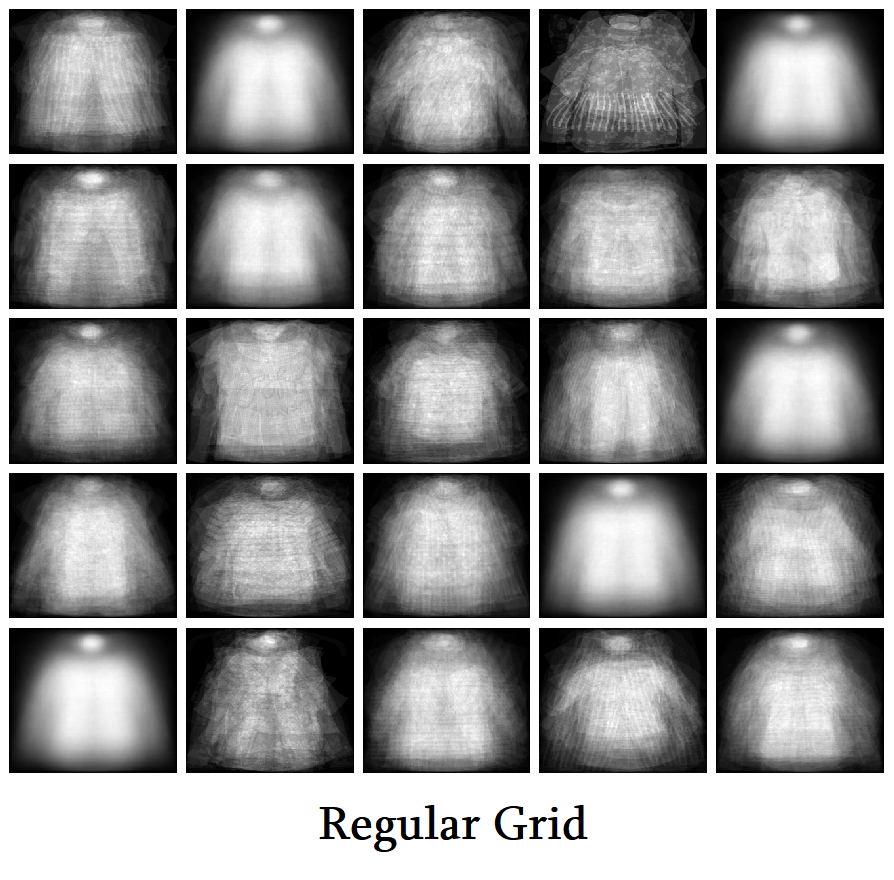
\includegraphics[width=.49\textwidth,height=250px]{./img/EM_RG}
	\end{figure*} 
	
	Risulta evidente, infatti, come l'algoritmo di clustering sia riuscito ad ottenere dei raggruppamenti soddisfacenti solo tramite i vettori ricavati dall'applicazione della prima tecnica. Dall'immagine di sinistra possiamo infatti distinguere numerosi tipi di abiti differenti come gonne, pantaloni (lunghi e corti), maglie a maniche lunghe e a maniche corte. Il clustering, in questo caso, è riuscito a differenziare anche tra abiti più stretti da altri più larghi. 
	Tutt'altra storia è quella raccontata dall'immagine di destra: il clustering, in questo caso, è stato fallimentare poiché, di tutte le immagini di media, non è presente una dalla sia possibile estrarre informazione ad alto livello. Le prestazioni non cambiano al variare di $k$.
	
	\section*{Mean Shift}
	
	L'algoritmo di Mean Shift è l'unico tra quelli utilizzati che non riceve come parametro il numero massimo di cluster da generare bensì il raggio $h$ della window che verrà utilizzata durante il processing del dataset. Per entrambi i tipi di features il parametro è stato posto a $h = 0,3$. Nel caso delle feature estratte tramite Bag of Words,  questa scelta (come nel caso precedente) è stata fatta ai fini della comparazione dei risultati e non per ottenerne di migliori. Anche in questo caso, infatti, Regular Grid (BoW) ha prodotto risultati non all'altezza di PCA.
	
	\begin{figure*}[ht!]
		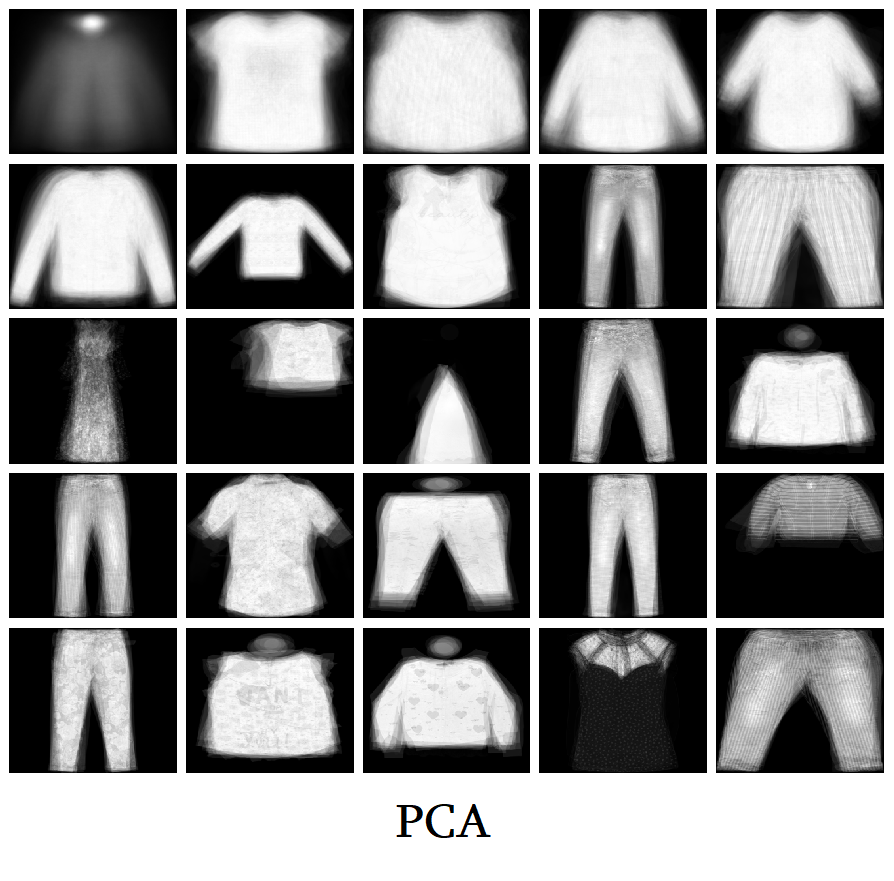
\includegraphics[width=.49\textwidth,height=250px]{./img/MS_PCA}\hfill
		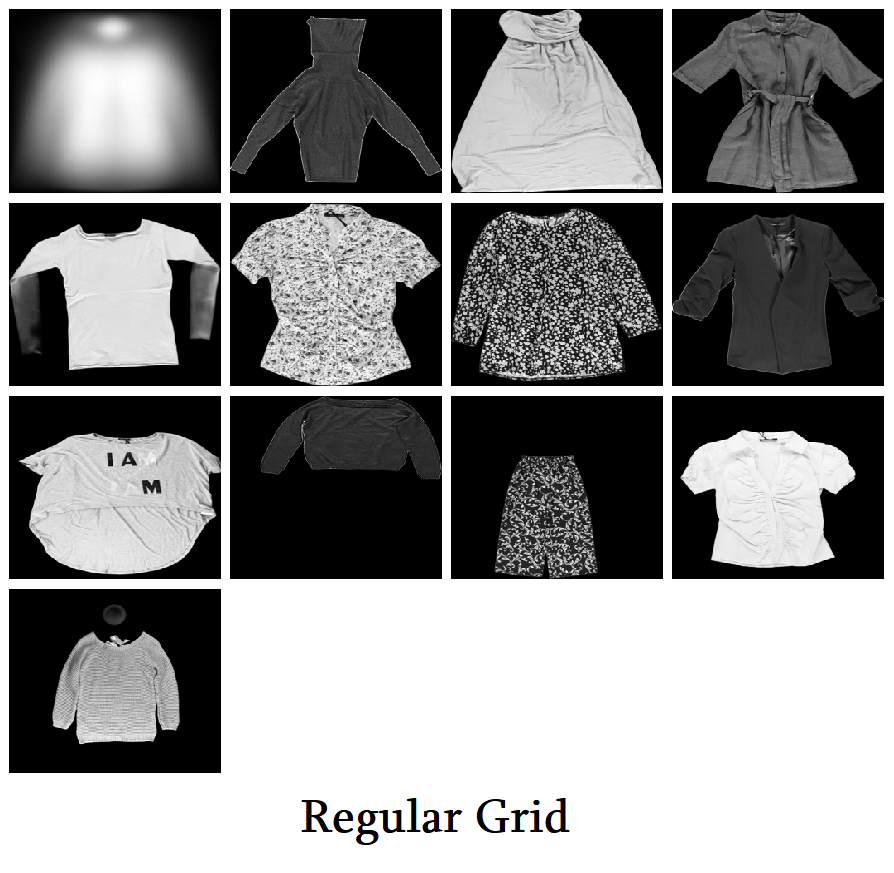
\includegraphics[width=.49\textwidth,height=250px]{./img/MS_RG}
	\end{figure*}
	
	Va sottolineato, però, che le immagini mostrate in figura relative a PCA rappresentano la media dei soli primi $25$ cluster individuati dall'algoritmo mean shift. In realta i cluster trovati sono stati molti di più e tra essi ve ne sono stati parecchi aventi cardinalità $1$ (come la quasi totalità dei cluster trovati con vettori relativi a BoW). Tuttavia, a destra, notiamo un importante differenza legata al fatto che tutte le immagini che non sono presenti in un cluster "singoletto" sono raggruppate in un unico cluster. Questo avviene principalmente per due cause:
	\begin{itemize}
		\item il valore di $h$ è troppo grande per il dataset in analisi e causa la creazione di un solo cluster interessante e tanti cluster "singoletti" relativi agli outliers;    
		\item i punti della distribuzione si concentrano tutti in una zona circoscritta e risulta impossibile distinguerli a causa dell'operazione di merge inserita nel codice di mean shift.
	\end{itemize}
	Nel caso in analisi è più probabile la seconda ipotesi poiché, al variare di $h$, i risultati non migliorano.
	Per quanto riguarda il raggruppamento ottenuto a sinistra ci si può comunque considerare soddisfatti poiché, pur essendo piccoli in termini di cardinalità, i cluster ottenuti contengono di certo immagini simili e dal soggetto chiaramente distinguibile.
	
	\section*{BSAS}
	
	I risultati ottenuti tramite BSAS sono stati sorprendentemente positivi nel primo caso  
	(applicazione dell'algoritmo al dataset ottenuto tramite PCA) mentre sono stati comicamente disastrosi nel secondo. 
	Anche in questo caso il parametro $k$ (numero massimo di cluster) è stato impostato a $25$ e in entrambi i casi questo è stato il numero effettivo di cluster restituiti. 
	
	Per quanto non sia netta come nei casi precedenti, è possibile individuare, nelle immagini di media a sinistra, la differenza tra gli abiti raggruppati in ogni cluster. Felpe e pantaloni lunghi sono gli indumenti che meglio sono stati caratterizzati da BSAS, meno uniformi sono i cluster che identificano t-shirt  e gonne/completi. Al di là di ciò, è stato interessante osservare come una tecnica di clustering così semplice riesca comunque ad arrivare a dei discreti risultati. 
	
	Analizzando le immagini di destra, quelle ottenute a partire dal dataset confezionato tramite BoW, salta subito all'occhio il primo cluster, per altro "singoletto", che individua una delle pochissime immagini di scarpe del dataset. Si evince dalla posizione dell'immagine che questo cluster è stato il primo ad essere generato: di conseguenza, l'outlier che ne fa parte, ha determinato la media del primo gruppo di immagini in maniera permanente. Dai restanti cluster non è possibile, di nuovo, ottenere alcun tipo di informazione. L'unico punto a favore di questo secondo dataset è il fatto che, dato in pasto a BSAS, ha permesso l'identificazione di un outlier conservandone quini l'informazione di "estraneità" anche durante la fase di estrazione delle features.

	\begin{figure*}[ht!]
		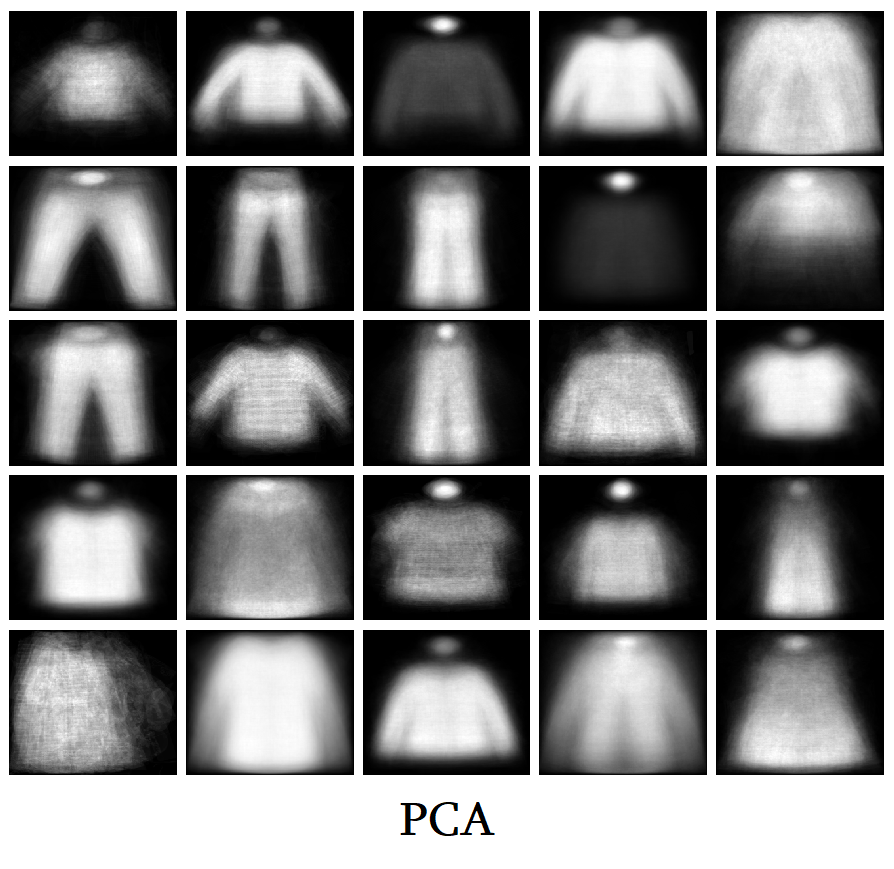
\includegraphics[width=.49\textwidth,height=250px]{./img/BSAS_PCA}\hfill
		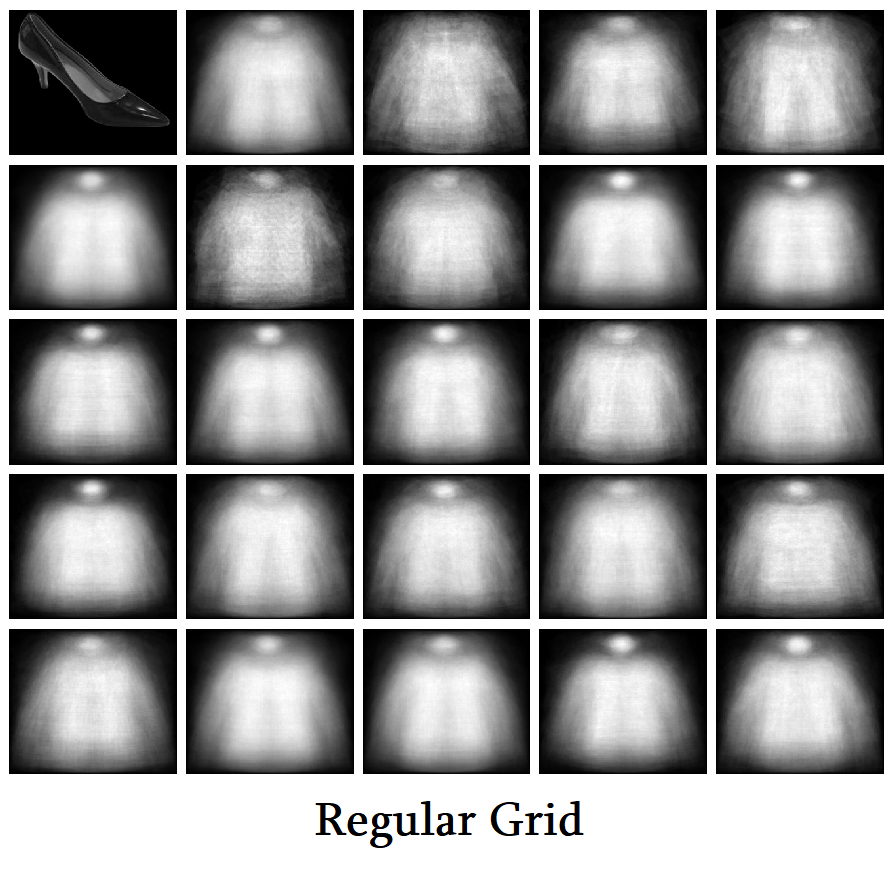
\includegraphics[width=.49\textwidth,height=250px]{./img/BSAS_RG}
	\end{figure*}

	
	\section*{Conclusioni}
	
	Dai risultati appena mostrati è possibile ricavare alcune considerazioni finali. 
	
	In particolare, è oramai chiaro come sia determinante, per una buona riuscita del clustering, il metodo utilizzato per estrarre le features dal dataset originale. Nel caso specifico si è dimostrata una certa superiorità di PCA rispetto a BoW (Regular Grid) per quanto riguarda l'estrazione di features interessanti dalle immagini processate. Va detto, ad onor del vero, che le ragioni dell'insuccesso di BoW sono individuabili nell'approccio che si è tenuto nei confronti del dataset stesso e nei parametri che si sono dati all'algoritmo. Infatti, per un applicazione efficace di questa tecnica, è fondamentale applicare preprocessing alle immagini, soprattutto se si usa una tecnica di estrazione delle parole che non gode di nessun tipo di invarianza (come nel nostro caso). Va inoltre considerato il fatto che i vettori risultanti dall'applicazione di BoW hanno features con valori interi e limitati ad un range ristretto. Questo range è stato reso probabilmente troppo piccolo a causa dell'imposizione all'algoritmo di parametri stringenti che ne consentissero la terminazione in tempi ragionevoli. 
	
	A conferma della scarso contenuto informativo dei vettori prodotti da BoW vi sono i risultati ottenuti con il clustering tramite Mean Shift. Tramite questi si può, infatti, avere un'idea sulla distribuzione dei punti nello spazio delle features. Avendo constatato che al variare della larghezza della window si ottiene sempre un cluster predominante che raggruppa la quasi totalità delle features, si può concludere che i sample si concentrino tutti in un certo intorno rendendo, in generale, difficile la creazione di cluster robusti.
	Per finire, un ruolo in questo contesto l'hanno giocato anche le word estratte che si sono rivelate poco adatte al loro scopo.
	
	I risultati ottenuti dal clustering del dataset estratto tramite PCA sono stati invece più convincenti. Tutti e tre gli algoritmi di clustering sono riusciti a trovare, in questo caso, dei raggruppamenti significativi. E' possibile riconoscere, per ciascun algoritmo, le principali classi di indumenti presenti nel dataset originale. Per questi casi l'operazione di clustering si può considerare conclusa con successo.  

\end{document}          